\section{Standard ISO/IEC 9126}\label{app:iso9126}
Lo standard norma un modello per la qualità del software descrivendone le caratteristiche. Si suddivide in :
\begin{itemize}
	\item \textbf{qualità in uso}: qualità per il prodotto finale quali efficacia, produttività, soddisfazione e sicurezza, di cui si avrà esperienza nella fase di utilizzo del prodotto;
	\item \textbf{qualità interna}: qualità della progettazione e del codice sorgente;
	\item \textbf{qualità esterna}: qualità in fase di test e di esecuzione.
\end{itemize}
Qualità esterna e qualità interna si suddividono ulteriormente nelle seguenti categorie di caratteristiche:
\begin{itemize}
	\item \textbf{Funzionalità}: soddisfacimento delle esigenze prestabilite attraverso
	\begin{itemize}
		\item \textbf{conformità}: adesione del prodotto a standard e convenzioni di funzionalità;
		\item \textbf{appropriatezza}: il prodotto offre funzionalità appropriate al soddisfacimento delle esigenze;
		\item \textbf{accuratezza}: il prodotto produce esiti congrui alle aspettative;
		\item \textbf{interoperabilità}: il software si integra correttamente nel sistema;
		\item \textbf{sicurezza}: il prodotto è robusto rispetto alle minacce esterne, non offre vulnerabilità.
	\end{itemize}
	\item \textbf{Affidabilità}: assicurare prestazioni nelle diverse circostanze. Comprende:
	\begin{itemize}
		\item \textbf{tolleranza agli errori}: il prodotto mantiene la consistenza interna rispetto alle modifiche autorizzate e ai malfunzionamenti;
		\item \textbf{maturità}: il prodotto è predisposto a non causare errori o  produrre esiti non corretti;
		\item \textbf{aderenza}: il prodotto è predisposto ad aderire agli standard e alle convenzioni;
		\item recuperabilità: a seguito di malfunzionamenti il prodotto è capace di riabilitare le prestazioni e ricostruire i dati colpiti da errori.
	\end{itemize}
	\item \textbf{Efficienza}: impiego di risorse ragionevoli nell'esecuzione delle sue attività. Include:
	\begin{itemize}
		\item \textbf{conformità}: adesione del prodotto a standard e convenzioni di efficienza;
		\item \textbf{utilizzo delle risorse}: congruo utilizzo delle risorse da parte del prodotto per il raggiungimento degli scopi prefissati;
		\item \textbf{comportamento rispetto al tempo}: il software produce risultati in un opportuno lasso di tempo.
	\end{itemize}
	\item \textbf{Usabilità}: grado di adoperabilità del prodotto, secondo:
	\begin{itemize}
		\item \textbf{conformità}: adesione del prodotto a standard e convenzioni di usabilità;
		\item \textbf{comprensibilità}: il prodotto è autoesplicativo o di facile utilizzo;
		\item \textbf{apprendibilità}: in che misura il prodotto richiede l'apprendimento di concetti per il suo utilizzo;
		\item \textbf{operabilità}: il prodotto richiede un certo grado di approntamenti per l'utilizzo;
		\item \textbf{attrattiva}: il prodotto genera una certa spinta al suo utilizzo.
	\end{itemize}	
	\item \textbf{Manutenibilità}: predisposizione alla correzione, all'adattamento e all'evoluzione. Ne fanno parte: 
	\begin{itemize}
		\item \textbf{analizzabilità}: il prodotto può essere ispezionato;
		\item \textbf{modificabilità}: il prodotto può essere modificato;
		\item \textbf{stabilità}: il prodotto è resiliente alle modifiche;
		\item \textbf{testabilità}: il prodotto può essere testato.
	\end{itemize}
	\item \textbf{Portabilità}: il prodotto mantiene le sue proprietà in qualsiasi sistema sia eseguito. Implica:
	\begin{itemize}
		\item \textbf{conformità}: adesione del prodotto a standard e convenzioni di portabilità;
	\item \textbf{installabilità}: il prodotto è disponibile in vari ambienti;
	\item \textbf{adattabilità}: il prodotto non richiede modifiche per il funzionamento in diversi ambienti ;
	\item \textbf{sostituibilità}: il prodotto utilizzato come alternativa ad un altro produce gli stessi risultati.
	\end{itemize}
\end{itemize}
\begin{figure}[H]
	\centering
	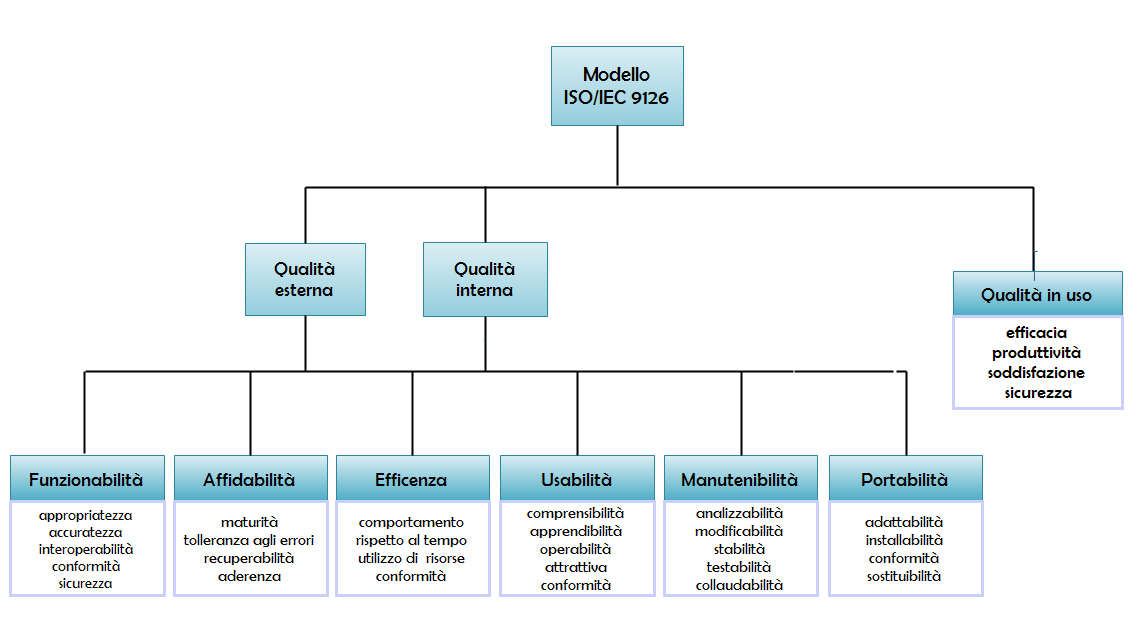
\includegraphics[width=15cm]{iso9126}
	\caption{Rappresentazione globale del modello \glossario{ISO}-\glossario{IEC} 9126}
\end{figure}